\section{Results}
\label{sec:results}
% GENERATED by scripts/real_results.py from repo files. Audit values are final; cost values are in progress (\prov).
\newcommand{\realAuditGemmaReported}{33.0}
\newcommand{\realAuditGemmaRecalc}{18.7}
\newcommand{\realAuditGptReported}{49.1}
\newcommand{\realAuditGptRecalc}{9.9}
\newcommand{\realAuditClaims}{40}
\newcommand{\realAuditReproduced}{31}
\newcommand{\realAuditContradicted}{2}
\newcommand{\realAuditNoArtifact}{7}
\newcommand{\realCostCalls}{\prov{122\,085}}
\newcommand{\realCostErrors}{\prov{655}}
\newcommand{\realCostLedgerMtok}{\prov{638}}
\newcommand{\realCostUsdLower}{\prov{84}}
\newcommand{\realCostWasteShare}{\prov{22}}
\newcommand{\realCostRitsShare}{\prov{96}}


This section compares every arm with the seed on three suites, prices the comparison, and then reports two measurements that justify the protocol: the operating characteristic of rule P and the audit of earlier CapEvolve gains.
\needs{One sentence with the headline result of the final evaluation: which arm leads on which suite, and by how much. Write it only after the numbers exist.}
Each difference is paired with the seed on the same tasks.
Intervals are family-cluster-robust, and p-values are Holm-adjusted within the suite (Section~\ref{sec:setup:stats}).
All arms are compared at the matched checkpoint $B^\ast$, the largest budget that every arm reached: \mockBstarA, \mockBstarB and \mockBstarC target rollouts on Suites A, B and C.
Red numbers with a dagger are placeholders that the final evaluation replaces, and orange numbers are real but still change while searches run.

\subsection{Suite A, SpreadsheetBench}
\label{sec:results:a}

On Suite A, \mockNsigA{} of the ten optimizer arms beat the seed with Holm-adjusted $p<0.05$, and the largest paired delta is \mockTopDeltaA{} points, held by \mockTopArmA{} (Table~\ref{tab:main_a}, Figure~\ref{fig:forest}).
The final set has \mockTA{} tasks, each scored with \mockTrialsA{} trials, for \mockSeedsA{} search seeds per arm.
\needs{State whether the CapEvolve arms are above, level with or below the best baseline, and whether their intervals exclude it.}
The one-shot control makes a single optimizer pass with no search, so it sets the floor that search must clear to justify its rollouts.
\needs{Report the one-shot control against the best search arm. If it is within one interval of the best arm, say that search adds nothing measurable here.}

\begin{table*}[t]
\centering
\scriptsize
\setlength{\tabcolsep}{3.5pt}
\caption{Suite A results, baselines by ascending delta and CapEvolve last, with the exploratory stock-gate arm below. Score is the final-set reward. $\Delta$ is the paired difference in points with a family-cluster-robust 95\% interval, $p_{\mathrm{Holm}}$ is Holm-adjusted within the suite, and USD is optimizer cost at Sonnet list prices. Missing is missing over scheduled cells. Tokens and wall clock are in Table~\ref{tab:cost_tokens}, per-seed values in Table~\ref{tab:perseed}, promotions per search in Table~\ref{tab:promotions}. Suite A has no one-shot control. The stock-gate arm (E12A on Suite A, E12C on Suite C) is exploratory and outside the Holm family. (placeholder)}
\label{tab:main_a}
\begin{tabular}{lcccrrr}
\toprule
Arm & Score (\%) & $\Delta$ vs seed [CI] & $p_{\mathrm{Holm}}$ & USD & Missing \\
\midrule
\multicolumn{6}{l}{\textit{Suite A, SpreadsheetBench verified-400 (Gemma-4-31B-it)}} \\
\midrule
Seed (no search) & \pend{50.0} & ref. & -- & -- & \pend{0/140} \\
Meta-Harness & \pend{51.1} & \pend{+1.1 [$-$5.8, +8.0]} & \pend{1.000} & \pend{28} & \pend{0/210} \\
EvoSkill & \pend{52.2} & \pend{+2.2 [$-$4.6, +9.0]} & \pend{1.000} & \pend{17} & \pend{4/210} \\
GEPA & \pend{53.3} & \pend{+3.3 [$-$2.7, +9.4]} & \pend{1.000} & \pend{7} & \pend{5/210} \\
Trace2Skill & \pend{55.2} & \pend{+5.2 [$-$1.6, +12.0]} & \pend{0.687} & \pend{18} & \pend{0/210} \\
MIPROv2 & \pend{55.5} & \pend{+5.5 [$-$0.6, +11.6]} & \pend{0.496} & \pend{11} & \pend{1/210} \\
ACE & \pend{55.8} & \pend{+5.8 [+0.3, +11.3]} & \pend{0.290} & \pend{16} & \pend{5/210} \\
WikiSkill (community) & \pend{55.9} & \pend{+5.9 [$-$0.7, +12.5]} & \pend{0.496} & \pend{6} & \pend{1/210} \\
SkillOpt & \pend{56.7} & \pend{+6.7 [+0.3, +13.1]} & \pend{0.290} & \pend{10} & \pend{1/210} \\
CapEvolve HC & \pend{53.4} & \pend{+3.4 [$-$3.5, +10.3]} & \pend{1.000} & \pend{27} & \pend{5/210} \\
CapEvolve AO & \pend{53.6} & \pend{+3.6 [$-$3.4, +10.6]} & \pend{1.000} & \pend{36} & \pend{9/210} \\
CapEvolve HC, stock gate \textit{(exploratory)} & \pend{54.4} & \pend{+4.4 [$-$2.1, +10.9]} & -- & \pend{37} & \pend{8/210} \\
\bottomrule
\end{tabular}
\end{table*}


\subsection{Suites B and C, tau2 retail and airline}
\label{sec:results:bc}

Suite B gives the cleaner second test, because its \mockTB{} test tasks are sealed (Table~\ref{tab:main_bc}).
There the largest paired delta is \mockTopDeltaB{} points (\mockTopArmB), and \mockNsigB{} arms clear Holm-adjusted $p<0.05$.
Suite C reuses the official airline test set of \mockTC{} tasks, which earlier work optimized against, so we call it development-exposed and do not rank arms on it.
Its largest delta is \mockTopDeltaC{} points (\mockTopArmC), and \mockNsigC{} arms clear $p<0.05$.
Even at 40 tasks the simulated minimum detectable effect of a single comparison is 0.10 to 0.13 under our planning assumptions (\texttt{analysis/out/sim\_mde.md}), and Suite C has half as many, so we read it descriptively.
\needs{State whether the arm ordering on B and C agrees with Suite A, using rank correlation of the paired deltas.}

\begin{table*}[t]
\centering
\scriptsize
\setlength{\tabcolsep}{3.5pt}
\caption{Suites B and C results. Columns as in Table~\ref{tab:main_a}. (placeholder)}
\label{tab:main_bc}
\begin{tabular}{lcccrrr}
\toprule
Arm & Score (\%) & $\Delta$ vs seed [CI] & $\Delta$ vs one-shot [CI] & $p_{\mathrm{Holm}}$ in family & USD & Missing \\
\midrule
\multicolumn{7}{l}{\textit{Suite B, $\tau^2$ retail, sealed test-40 (gpt-oss-120b)}} \\
\midrule
\multicolumn{7}{l}{\textit{Reference arms}} \\
Seed (no search) & \pend{55.0} & ref. & \pend{$-$2.7} & -- & -- & \pend{2/120} \\
One-shot control & \pend{57.7} & \pend{+2.7 [$-$6.4, +11.7]} & ref. & \pend{1.000} & \pend{2} & \pend{5/360} \\
\multicolumn{7}{l}{\textit{Competitors, secondary family}} \\
GEPA & \pend{57.5} & \pend{+2.5 [$-$6.2, +11.2]} & \pend{$-$0.1 [$-$9.7, +9.6]} & \pend{1.000} & \pend{10} & \pend{6/360} \\
HarnessLens & \pend{61.6} & \pend{+6.6 [$-$0.5, +13.6]} & \pend{+3.9 [$-$3.9, +11.8]} & \pend{0.521} & \pend{15} & \pend{2/360} \\
\multicolumn{7}{l}{\textit{CapEvolve, primary family}} \\
CapEvolve HC & \pend{57.2} & \pend{+2.2 [$-$5.5, +9.8]} & \pend{+1.1 [$-$7.5, +9.6]} & \pend{1.000} & \pend{46} & \pend{9/360} \\
CapEvolve AO & \pend{55.3} & \pend{+0.3 [$-$7.7, +8.3]} & \pend{+0.6 [$-$8.3, +9.6]} & \pend{1.000} & \pend{33} & \pend{0/360} \\
\midrule
\multicolumn{7}{l}{\textit{Suite C, $\tau^2$ airline, official test-20 (development-exposed)}} \\
\midrule
\multicolumn{7}{l}{\textit{Reference arms}} \\
Seed (no search) & \pend{40.0} & ref. & \pend{+3.6} & -- & -- & \pend{2/60} \\
One-shot control & \pend{36.4} & \pend{$-$3.6 [$-$17.9, +10.8]} & ref. & \pend{1.000} & \pend{3} & \pend{2/180} \\
\multicolumn{7}{l}{\textit{Competitors, secondary family}} \\
HarnessLens & \pend{42.0} & \pend{+2.0 [$-$11.5, +15.4]} & \pend{+4.1 [$-$10.4, +18.6]} & \pend{1.000} & \pend{6} & \pend{0/180} \\
GEPA & \pend{44.1} & \pend{+4.1 [$-$6.6, +14.9]} & \pend{+8.9 [$-$2.7, +20.5]} & \pend{1.000} & \pend{13} & \pend{8/180} \\
\multicolumn{7}{l}{\textit{CapEvolve, primary family}} \\
CapEvolve HC & \pend{40.0} & \pend{+0.0 [$-$14.3, +14.3]} & \pend{+9.9 [$-$5.5, +25.3]} & \pend{1.000} & \pend{31} & \pend{3/180} \\
CapEvolve AO & \pend{43.9} & \pend{+3.9 [$-$9.9, +17.7]} & \pend{+9.2 [$-$5.7, +24.0]} & \pend{1.000} & \pend{16} & \pend{0/180} \\
\multicolumn{7}{l}{\textit{Exploratory, outside the Holm family}} \\
CapEvolve HC, stock gate & \pend{44.9} & \pend{+4.9 [$-$8.4, +18.2]} & \pend{+8.6 [$-$5.7, +23.0]} & -- & \pend{36} & \pend{1/180} \\
One-shot best of $k$ & \pend{44.5} & \pend{+4.5 [$-$7.1, +16.0]} & \pend{+8.0 [$-$4.5, +20.5]} & -- & \pend{23} & \pend{9/180} \\
\bottomrule
\end{tabular}
\end{table*}


\begin{figure*}[t]
\centering
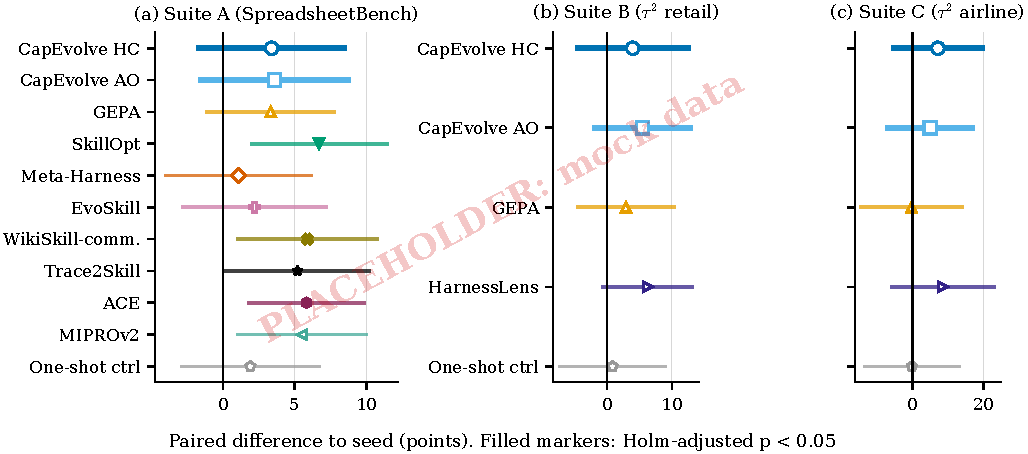
\includegraphics[width=\textwidth]{figures/fig_forest.pdf}
\caption{Paired delta to the seed, per suite, with 95\% intervals. CapEvolve arms are drawn thick. Filled markers have Holm-adjusted $p<0.05$. An interval that crosses zero is not evidence of a gain (placeholder).}
\label{fig:forest}
\end{figure*}

\subsection{Cost}
\label{sec:results:cost}

Arms differ in what they spend, and the tables report optimizer tokens in three classes because cache reads and cache writes are priced differently from uncached input.
Figure~\ref{fig:pareto} plots delta against cost and Figure~\ref{fig:anytime} plots score against rollouts, both in Appendix~\ref{app:results}.
\needs{Say which arms lie on the cost-quality frontier on each suite, and whether the frontier changes between USD and tokens as the cost axis.}
Across the whole campaign the gateway has metered \realCostCalls{} calls and \realCostLedgerMtok{} million ledger tokens, and \realCostWasteShare{}\% of those tokens went to smoke tests, restarts and superseded runs.
These count toward campaign cost but toward no arm's cost in the tables.
The metered optimizer spend at Sonnet list prices is at least \$\realCostUsdLower{}, a lower bound because RITS and GPT-5.5 calls have no price available to us.
Table~\ref{tab:cost_so_far} gives the per-arm breakdown and Figure~\ref{fig:roles} the split by role.

\subsection{Rule P cuts false promotion and costs power}
\label{sec:results:p}

In simulation, rule P (Section~\ref{sec:method:P}) promotes a null candidate far less often than the one-stage gate, and it promotes a real improvement less often too (Figure~\ref{fig:rulep}).
With the campaign setting (three confirmation trials, $z=1.282$), a search of six all-null candidates produces at least one false promotion with probability 0.050, against 0.434 for the one-stage gate with $k=1$ and 0.199 with $k=1.645$.
For a single candidate with a true effect of ten points, rule P promotes it with probability 0.41 and the one-stage $k=1$ gate with probability 0.54.
The simulations run the real gate code (\texttt{analysis/out/sim\_budget.md}).
They show the trade, not an improvement in final scores.
\needs{Add the E12 ablation (one-stage gate against rule P) once its final evaluation exists, or state that the campaign has no such ablation.}

\subsection{Most of the historical gain was scorer compliance}
\label{sec:results:audit}

Recomputed under the SpreadsheetBench recalculation scorer, the historical CapEvolve gains shrink from +\realAuditGemmaReported{} to +\realAuditGemmaRecalc{} points on Gemma-4-31B and from +\realAuditGptReported{} to +\realAuditGptRecalc{} points on GPT-5.5 (Figure~\ref{fig:audit}).
The historical scorer reads the workbook as saved, so a model that writes a value in place of a formula passes.
Both scorers were applied to the same output files, so each comparison is fair inside its scorer, but most of the as-saved gain is compliance with a scoring convention and not task skill.

The arithmetic was mostly right.
Of \realAuditClaims{} recomputed claims, \realAuditReproduced{} reproduce to the decimal, \realAuditContradicted{} are contradicted in framing and \realAuditNoArtifact{} have no artifact that produces them (Table~\ref{tab:audit}).
One contradiction matters for the comparison with simpler methods: a hill-climb control from the same empty seed reached 85.6 on the same test tasks where the headline agent-optimize run reached 76.4, and the earlier write-up omitted it.
Earlier optimizer runs had also seen the test sets, so no clean split remained, which is why Suites A and B use fresh final sets.
No historical number appears in the result tables.

\begin{figure*}[t]
\centering
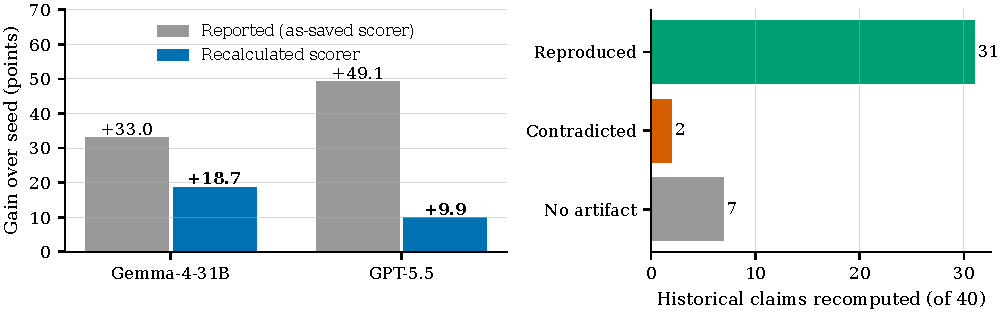
\includegraphics[width=\textwidth]{figures/fig_audit.pdf}
\caption{Recalculation removes most of the historical gain. Left: reported and recalculated gains of the two SpreadsheetBench headline runs. Right: outcome of recomputing every historical claim from archived artifacts (\texttt{audit/recomputed\_numbers.csv}).}
\label{fig:audit}
\end{figure*}

\begin{table}[t]
\centering
\scriptsize
\caption{Selected historical claims and their recomputation from archived artifacts (40 claims in total).}
\label{tab:audit}
\begin{tabularx}{\columnwidth}{@{}p{0.9in}X@{}}
\toprule
Claim & Recomputation \\
\midrule
Gemma +33.0 [29.1, 36.8] & reproduces; interval is pooled over observations, task-clustered is [26.9, 39.2]; +18.7 under recalculation \\
GPT-5.5 +49.1 [45.5, 52.8] & reproduces; recalculated gain is +9.9 \\
GPT-5.5 recalculated baseline 77.5 & reproduces; 110 of 217 recalculated passes need formulas \\
no-capability control 62.9 & same run's one-iteration hill climb scores 85.6, absent from the draft \\
run excluded for different commit & 55 of 280 rollouts hit a budget error; baseline 28.9 is on 225 tasks \\
SkillsBench 55.6 to 66.7 held out & the whole delta is one trial of one task \\
SWE-bench pilot 68.0, candidate 72.0 & candidate rejected; the seed scores 63.6 and 70.5 on the same 44 tasks \\
$\tau^2$ retail 0.460 to 0.545 & arithmetic only; no per-task artifact exists \\
$\tau^2$ held-out 30.0 to 47.5 & artifact never landed; runner identity differs between docs \\
\bottomrule
\end{tabularx}
\end{table}


\subsection{Infrastructure incidents shaped what the data supports}
\label{sec:results:ops}

Five incidents changed the data, and Appendix~\ref{app:incidents} lists each with its effect.
Gateway priority was a hidden treatment: a stale low-priority tag kept EvoSkill rollouts queued from 13:05 to 18:40 UTC on the first day, so all its rollouts after 13:05 are invalid and its three seeds restarted from scratch.
EvoSkill was expected to finish about five and a half hours behind the other Tier 1 arms and so to bind $B^\ast$.
Gateway 502 errors hit 1 to 2.5\% of Gemma calls until a transparent retry went in at 13:11.
Before then, the shared adapter scored a failed rollout as zero for competitor arms but dropped it for CapEvolve, so the bias fell on competitors and grew with rollout length.
The retry is identical for every arm, and we report a sensitivity analysis that treats the earlier failures as missing.

Three more incidents were contained by restarts and policy.
The first Suite B launch used the wrong judge and no rule P, so we discarded it and relaunched.
Hung rollouts, up to 114 minutes on ACE and MIPROv2, led to one rule for all arms: a timeout is an infrastructure error with one retry, counted outside the rollout budget, and never reward zero.
ACE and HarnessLens needed prompt and retry changes recorded as deviations.

One isolation gap remains open and disclosed.
On Suite B, the CapEvolve optimizer could initially read the task file with gold actions, including the sealed test tasks.
We relaunched both arms inside a mount-namespace shim, and a scan of every earlier optimizer transcript found no read of the task files.
The agent-optimize arm still runs the evaluator in its own shell, so its sandbox holds gold actions for its 74 optimization and selection tasks, never for the sealed test set.
Selection-time comparisons for that arm on Suite B are flagged for that reason.
